

\documentclass[DM,authoryear,toc,lsstdraft]{lsstdoc}
% lsstdoc documentation: https://lsst-texmf.lsst.io/lsstdoc.html

% Package imports go here.
\usepackage{graphicx}

% Local commands go here.

% To add a short-form title:
% \title[Short title]{Title}
\title[Solar System Data Products Changes]{Proposed Modifications to Solar System Processing and Data Products}

% Optional subtitle
% \setDocSubtitle{A subtitle}

\author{%
Mario Juric,
Siegfried Eggl,
Joachim Moeyens
and Lynne Jones
}

\setDocRef{DMTN-087}

\date{\today}

% Optional: name of the document's curator
\setDocCurator{Mario Juric}

\setDocAbstract{%
A high-level presentation of proposed changes to Solar System processing and data products baseline, to bring LSST Solar System processing closer to common asteroid-survey workflows, and help the on-schedule delivery of a scientifically useful set of Solar System data products.
}

% Change history defined here.
% Order: oldest first.
% Fields: VERSION, DATE, DESCRIPTION, OWNER NAME.
% See LPM-51 for version number policy.
\setDocChangeRecord{%
  \addtohist{1}{2018-06-22}{2018 Review Release.}{Mario Juric}
  \addtohist{2}{2019-07-XX}{Serving as RFC/LCR summary.}{Mario Juric}
}

\begin{document}

% Create the title page.
% Table of contents is added automatically with the "toc" class option.
\maketitle

% ADD CONTENT HERE

\section{Introduction}

Taking the inventory of the Solar System is one of the four main science themes that LSST is designed to enable. As \cite{2008arXiv0805.2366I} discuss:

\begin{quotation}
The small bodies of the Solar System, such as main belt
asteroids, the Trojan populations of the giant planets
and the Kuiper Belt objects, offer a unique insight
into its early stages because they provide samples of
the original solid materials of the solar nebula. Understanding
these populations, both physically and in their
number and size distribution, is a key element in testing
various theories of Solar System formation and evolution.

The baseline LSST cadence will result in orbital parameters
for several million objects; these will be dominated
by main-belt asteroids, with light curves and
multi-color photometry for a substantial fraction of detected
objects. The LSST sample of asteroids with accurate
orbits and multi-color light curves will be 10 to
100 larger than currently available sample. LSST will
make a significant contribution to the Congressional target
completeness of 90\% for PHAs larger than 140m, and will 
detect over 30,000 TNOs brighter than r ∼ 24.5 using 
its baseline cadence. LSST will be capable
of detecting objects like Sedna to beyond 100 AU,
thus enabling in situ exploration far beyond the edge of
the Kuiper belt at ∼50 AU. Because most of these objects
will be observed several hundred times, accurate
orbital elements, colors, and variability information will
also be available.
\end{quotation}

Consistent with the overall data products strategy derived from the \citeds[SRD]{LPM-17},
LSST DM has identified Solar System-oriented products and 
processing that would be i) {\em broadly useful} and ii) that 
{\em LSST is uniquely position to deliver}\footnote{i.e., where community-led
creation of such products would be infeasible due to technical
constraints (such as bandwidth or computing required), or where
the creation of products would require a high-degree of LSST-specific
expert knowledge unlikely to be readily available in the community
(such as understanding of instrumental artefacts or the details of
LSST software).}.

Applied to the Solar System science theme, this overall guidance led us to 
articulate three specific data products desiderata:
%
\begin{enumerate}
	\item Enable real-time ($\sim$minutes) identification of fast-moving solar system object candidates. The goal is to facilitate discovery and rapid follow-up of objects in close proximity to Earth.
	\item Enable real-time attribution of new observations of known Solar System objects. This facilitates identification of uncommon (i.e., cometary) activity on otherwise known objects, but also reduces the chance an asteroid may be mistaken for a transient.
	\item Identify previously unknown solar system objects (those moving on orbits around the Sun), and associate (group) together their repeated observations. This facilitates the census of the Solar System, studies of physical and dynamical properties of individual bodies, as well as studies object populations.
\end{enumerate}


\section{Present Baseline}

The LSST data products baseline \citedsp[DPDD]{LSE-163} has been constructed to respond to the desiderata of all LSST science themes, including the Solar System desiderata enumerated in the previous section. This baseline is described in detail in the DPDD; we only give a brief summary here, concentrating on Solar System science.

\begin{enumerate}
	\item To satisfy the real-time identification of fast-moving candidate Solar System objects, we have added the fitting of Trailed Source Model to every DIASource detection. The resulting measurements will be transmitted in the event alert stream.
	\item To satisfy the need for real-time attribution, we compute predicted positions (ephemerides) of known objects at time of each observation, and associate observations (DIASources) detected at those positions. We use an internally maintained orbit catalog (see next item), as well as an external catalog (MPCORB). The associations are also transmitted in the real-time event alert stream.
	\item To identify previously unknown objects, we are developing an LSST-specific version of the MOPS pipeline \citedsp[LDM-156]{LDM-156}. Orbits are computed for all newly discovered objects, and are added to the LSST orbit catalog (the "SSObject" table). This catalog's primary purpose is to enable attribution of subsequently (and previously) detected DIASources to LSST-discovered Solar System objects. It is also made public, on a daily basis, together with some useful pre-computed physical properties (e.g., absolute magnitudes in LSST bands).
	\item Finally, to enable an accurate census of the Solar System, we repeat the MOPS-driven detection procedure and object catalog construction for each LSST Data Release. These catalogs are produced with a single, well-characterized, version of MOPS, and validated more extensively than the daily versions. The Data Release catalogs also benefit from the improved astrometry and photometry available in data releases.
\end{enumerate}

In summary: objects with motions sufficient to cause trailing in a single exposure will
be identified and flagged as such when the alerts are broadcast. Those that are not trailed will be identified and linked based on their motion from observation to observation, over a period of a few days. Their orbits as derived by MOPS will be published within 24 hours of identification. Better characterized object catalogs, suitable for population studies, will be computed and published with each Data Release. The daily aspect of this production is illustrated in Figure~\ref{fig:productionNow}.

\begin{figure}
	\caption{A simplified view of nightly production of Solar System related products.\label{fig:productionNow}}
	\centering
	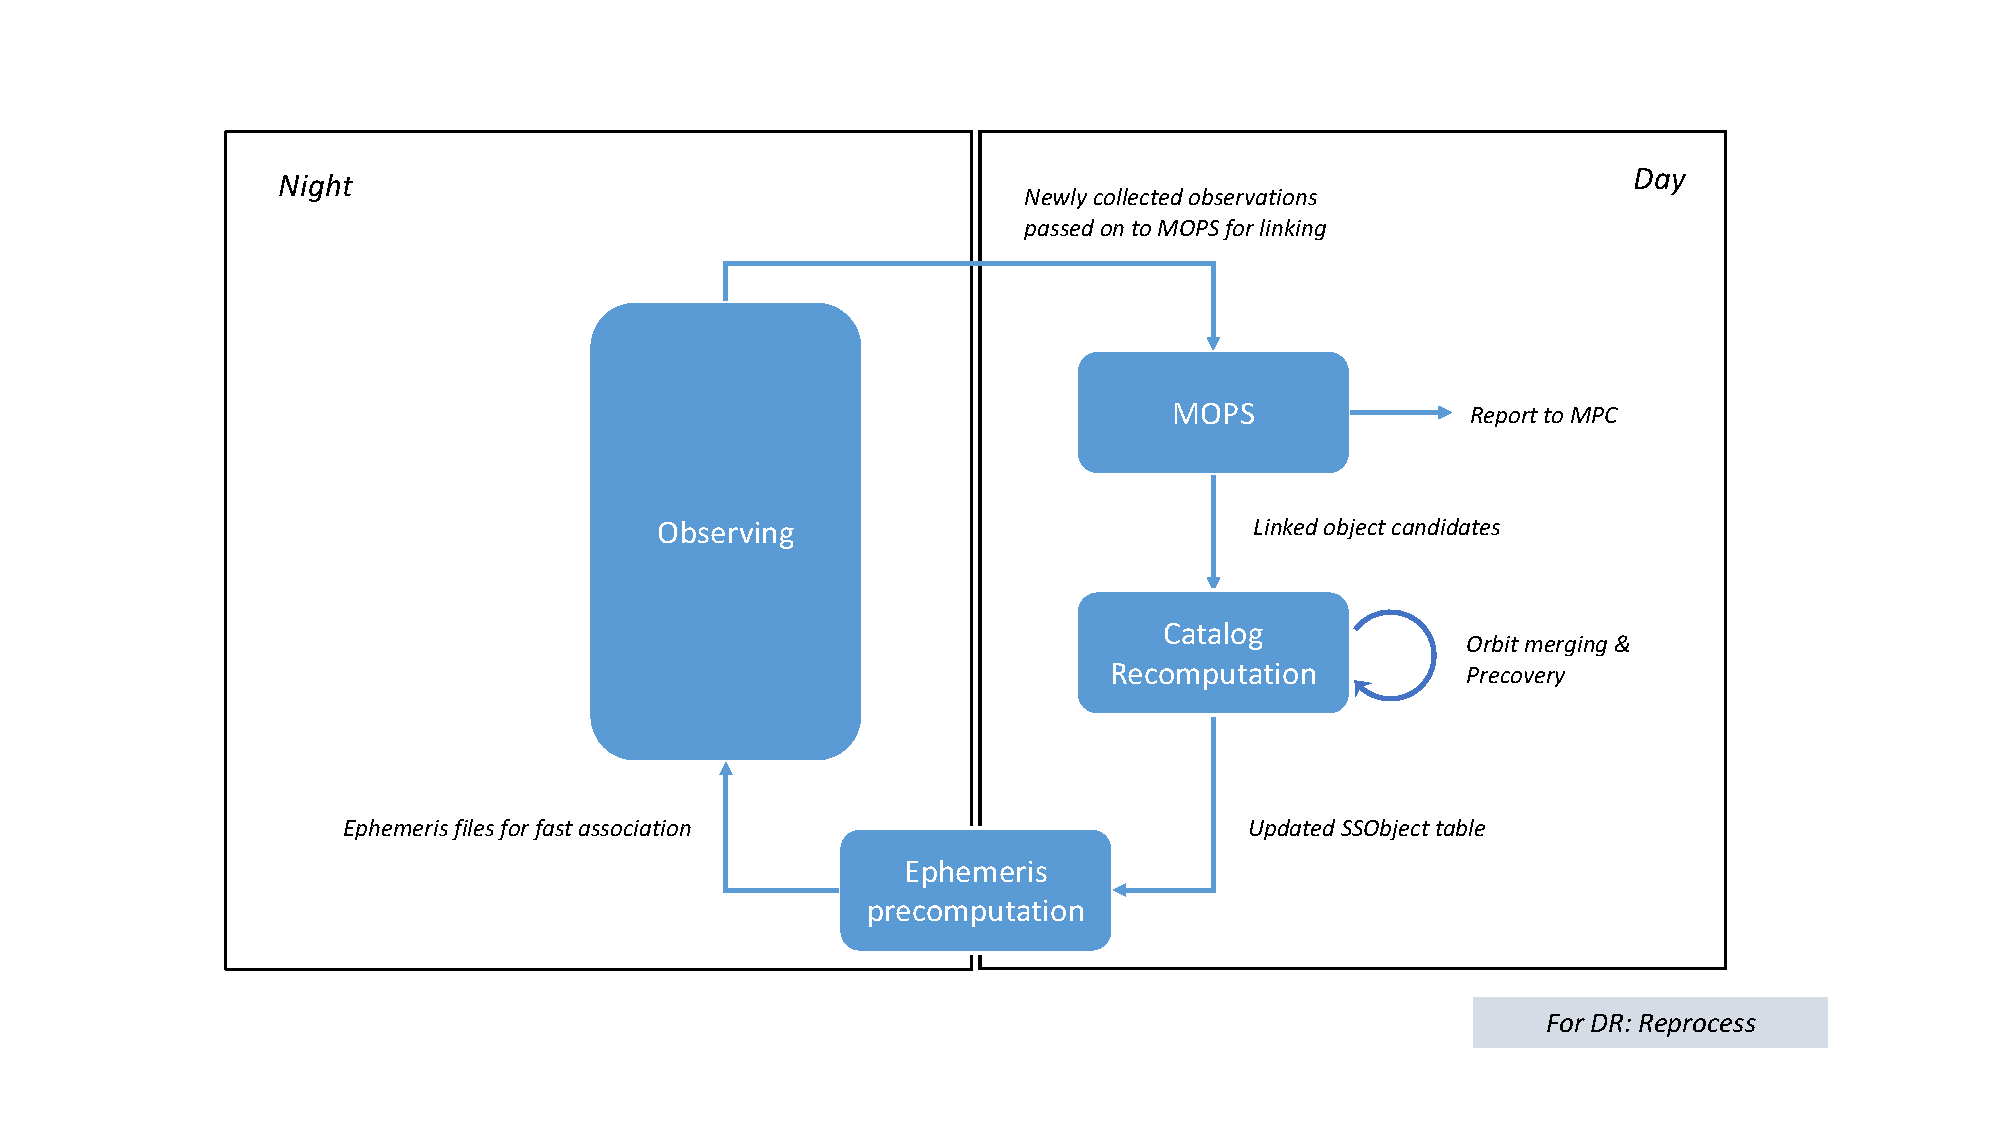
\includegraphics[page=1,width=1.0\textwidth]{figures/processing.pdf}
\end{figure}

\section{Issues}

The described data product baseline has been reviewed and adopted in 2013. Since then, a number of issues have been identified that caused us to re-examine some of the adopted solutions. We discuss them from the point of view of scientific usability (scope), the development schedule, and the development budget (cost).

\subsection{Science}

Though the baseline presented in previous section satisfies the desiderata for the Solar System science related products, we have identified elements that can be improved. Specifically:

\begin{itemize}
	\item The current scheme requires associating every newly observed source (a DIASource) with two independently maintained catalogs: the internal LSST orbit catalog, and an external (Minor Planet Center; MPC) catalog\footnote{The association with an external catalog is necessary to maximize completeness, especially early on in the survey.}. A consequence is that each object would have both an LSST ID and/or a MPC designation. These designations may sometimes be in conflict: e.g., the LSST catalog may attribute two observations to two different (typically short-arc) objects, while the MPC catalog may attribute them to the same object (given it generally has access to more data than LSST). Though not insurmountable, these types of ``bookkeeping'' issues will make it more difficult to work with the LSST catalog.
	\item Presently there are no plans to cross-reference the LSST catalog to the MPC catalog.
As a consequence, the end-users will have to do this type of orbit-to-orbit matching themselves, which may be rather non-trivial (especially in the case of short-arc orbits).
	\item Finally, tracklets that are not linked by LSST MOPS are never reported to the Minor Planet Center. Therefore, objects that could be discovered by linking LSST's tracklet to one from another survey will be lost.
\end{itemize}
	
\subsection{Budget}

%We have examined the present development status and resources assigned to construction and commissioning of the Solar System software components (MOPS).

The present baseline for the development and commissioning of MOPS has budgeted for 3 FTE-years of graduate student effort, 1 FTE-yr of postdoctoral fellow effort, and 0.75 FTE-years of supervisory faculty effort. Having recently re-examined the the state of the software prototypes inherited from R\&D, and with better modeling of development team productivity, we believe is not possible to deliver the products as presently envisioned with the resources available.

Instead, in Section~\ref{sec:new}, we will present potential modifications to the products and processing strategy. These retain the scientific value while reducing the resources needed to construct the processing software.

\subsection{Schedule\label{sec:schedule}}

The present development plan assumed full engagement on MOPS construction starting in 2017. As hiring in this area is difficult, the actual work lagged relative to the plan.

It's unlikely we could restore this schedule by adding significantly more people at this phase of the project\footnote{This is commonly known as Brooks' Law: ``adding human resources to a late software project makes it later'' \citep{1982mmme.book.....B}}. A better strategy may be to re-examine the work to be done, with a goal of simplifying the design while retaining most (or all) of the scope (while continuing to make well-suited hires, if possible). We discuss such a proposal in Section~\ref{sec:new}.

\subsection{Operational Considerations}

The presently defined scope calls for daily production of an updated orbit catalog. This process is largely automated, but it has been known to occasionally require manual intervention by a domain-expert (curation). This is especially true when it comes to incorporation into the orbit database of numerous newly discovered short-arc objects. The Minor Planet Center dedicates approximately $\sim$2 FTE to maintenance of a comparable catalog.

At present, plans for LSST operations do not explicitly include staff with Solar System / orbital dynamics expertise to fulfill this type of role. This carries a significant operational risk, should the orbit catalog maintenance code not be sufficiently autonomous.

\section{Overview of Proposed Changes\label{sec:new}}

The issues described in the previous section point to serious obstacles to an on-schedule delivery of the LSST Solar System Data Products, as presently envisioned. We have therefore holistically re-examined the deliverables in this area, looking for redesign opportunities to allow for deliver close to desired schedule, with a minimum impact to the budget.

\subsection{Processing Workflow\label{sec:promptSSP}}

Before looking at LSST, it is instructive to sketch out how analogous present-day asteroid surveys operate. We take the example of a typical night in PanSTARRS: i) observations are taken, ii) known objects are flagged by comparing detections to external catalogs (MPCORB), iii) tracklets are constructed by PS1-MOPS, iv) likely asteroids are submitted to the Minor Planet Center (MPC), v) the Minor Planet Center confirms the detections and (where possible) computes and publishes orbits in time for the next night of observing.
Comparing this workflow to Figure~\ref{fig:productionNow}, we see that this closely follows the model adopted by LSST. The major difference is that all the steps in the LSST processing are performed in-house, whereas PS1 relies on the Minor Planet Center.

The Minor Planet Center\footnote{\url{https://www.minorplanetcenter.net/iau/mpc.html}} (MPC) operates at the Smithsonian Astrophysical Observatory (SAO), under the auspices of Division F of the International Astronomical Union (IAU). The MPC is responsible for the designation of minor bodies in the solar system: minor planets; comets; and natural satellites. They are also responsible for the efficient collection, computation, checking and dissemination of astrometric observations and orbits for minor planets and comets, via its various journals. The MPC was founded at the University of Cincinnati in 1947, and has been operating at the SAO since 1978. Reporting small body discoveries to the MPC, who construct and curate the resulting orbit catalogs, has been an established community practice at least since the $\sim$1970s.

The rationale for LSST not utilizing MPC services are largely historical. When LSST was originally envisioned, the Minor Planet Center infrastructure was not going to scale to the sheer volume of data LSST was predicted to produce\footnote{LSST was originally designed to begin operating in early 2010s.}. Furthermore, keeping full control over all aspects of the processing minimized operational risk.

The LSST start date has shifted by a $\sim$decade since these original designs. In this time, the predicted data volumes for LSST have stayed the same, while the generally available computing capabilities have increased. The MPC has demonstrated the ability to scale with the growth of the community (e.g., it successfully handles PanSTARRS PS1 data). Today, the MPC routinely manages a database of $\sim 750,000$ orbits, only a factor of $\sim 7$ relative to what is expected for end-of-mission LSST.

We've therefore examined the elements in Figure~\ref{fig:productionNow} with the aim of bringing LSST Solar System processing closer to present day practices that utilize Minor Planet Center services. There are two major sources of Solar System-specific pipelines (in terms of construction and operations effort):
\begin{enumerate}
	\item Delivering the MOPS pipeline to link tracklets into high-probability candidate tracks
	\item Delivering the pipeline to construct, manage, and maintain (in operations) the resulting orbit catalog.
\end{enumerate}
The specific method that LSST adopted for discovery and linking of solar system objects requires a MOPS pipeline with a computationally intensive ``link tracklets'' step. The novelty of the method, and the sheer computational intensity, argue for continued in-house development of this step.

\begin{figure}
	\caption{A simplified view of nightly production of Solar System related products, with orbit catalog generation and curation performed by the Minor Planet Center. A detailed workflow can be found in Figure~6 of LDM-151.\label{fig:productionNew}}
	\centering
	\includegraphics[page=2,width=1.0\textwidth]{figures/processing.pdf}
\end{figure}

The second step -- construction and maintenance of the orbit catalog -- is an example of ``bread and butter'' operation that the MPC specializes in. If LSST delivered a list of already linked tracklets, the MPC has the software, staff,  processes, and capabilities to ingest them, verify the linkage, add them to the orbit database, and perform all the typical curation activities. Assuming MPC services are used for this step, the resulting daily cycle is presented in Figure~\ref{fig:productionNew}.

By switching to the scheme presented in Figure~\ref{fig:productionNew}, the newly discovered high-confidence tracks would now be submitted to the MPC for inclusion into the central orbit database they maintain and regularly curate. Following incorporation of nightly data received from LSST and other surveys, the MPC would publish an updated orbit catalog in time for the next night of LSST observing. LSST would download the published catalog, and use it for attribution of known objects in the following night.

\subsection{Data Products}

From the data products point of view, the change can be viewed as having an SSObject table divided into two parts: dynamical and physical characteristics. The dynamical characteristics (orbital elements) would now be computed by the Minor Planet Center (the "MPCORB" catalog); LSST would ingest a new copy of the MPCORB every evening. We note that this means that {\bf the orbits in the ingested catalog will be computed using not only LSST observations, but also other observations the MPC has access to}. The biases, selection function, and the quality of orbits in the catalog will therefore be complicated, making this catalog unsuitable for population studies. The DRP catalogs (see below) should be used for this purpose.

Given that information, the physical characteristics such as absolute magnitudes would still be computed by LSST (also on a nightly basis, forming tne updated SSObject table). This is schematically illustrated in Figure~\ref{fig:productsComparison}.

\begin{figure}
	\caption{Comparison of present data products baseline, and the proposed changes. See text for details.\label{fig:productsComparison}}
	\centering
	\includegraphics[page=3,width=0.8\textwidth]{figures/processing.pdf}
\end{figure}

To facilitate the determination of biases LSST will, as a part of DRP, compute an orbit catalog and the table of physical properties using LSST observations only and utilizing one, well-characterized, version of the Solar System Processing pipeline. This products is designed to enable population studies based on objects discovered by LSST.

\subsection{Linking Algorithm}

A new tracklet linking algorithm, HelioLINC, has recently been published and demonstrated by \cite{2018AJ....156..135H}. This algorithm brings significant (>10x) computational improvements over the present baseline, as well as being conceptually simpler.

We have analyzed its linking performance. We find that present day implementation (\url{https://github.com/pytrax/pytrax}) is already able to link $> 90$\% of non-NEO objects and $> 70$\% of NEOs in a simulate 3-month LSST survey. Technical analysis of possible improvements indicates that with additional development (budgeted in this change request) this codebase can be updated to meet LSST requirements ($95$\% linking efficiency). The computational performance is approximately $10$x over the present LSST MOPS prototypes.

Given the new algorithm's simplicity, increased computational performance, and the ability to share code and know-how with the Minor Planet Center (the original developers), we propose to switch to HelioLINC as the baseline linking algorithm.

\section{Impact Assessment}

\subsection{Science}

Our analysis and feedback from the LSST Solar System Science Collaboration indicates this change will have an overall positive impact. It will lead to improved usability, asteroid characterization, and enhanced discovery yields. Specific benefits include:
%
\begin{itemize}
\item As MPCORB includes not only LSST information, but other surveys as well, the orbit catalog used for association is now maximally complete at all times. This also automatically satisfies DMS-REQ-0288 ("Use of External Orbit Catalogs").
\item There is now only one catalog now (a opposed to having an LSST-specific orbit catalog). This solves the non-trivial cross-match problem, simplifies bookkeeping, and reduces community confusion.
\item For the community that already works with the MPC databases, there will be no need to do anything special to take advantage of LSST data (as it will already be included). This makes the LSST measurements significantly more accessible and useful.
\item This change places LSST into a more general (and already largely existing) framework of how asteroid surveys operate
world-wide
\item The change would open the possibility to submit all tracklets to the MPC, including trails
\item The change would enable future cross-survey linking either at MPC or by a third party. For example, LSST’s first tracklet may complete a track that some other survey has started nights before. This increases the overall object discovery yields.
\end{itemize}

On the negative side, not having an LSST-only nightly catalog diminishes its value for precision population studies. However, the data release catalogs are arguably better (and specifically designed) for that use case.

\subsection{Budget and Schedule}

We estimate that with this change the construction scope of prompt Solar System processing can be executed with the presently hired staff in time for the beginning of operations. We estimate the DRP elements will be possible to construct in the same time-frame {\em assuming no significant changes are needed to prompt processing elements as a result of feedback from commissioning.}

A secondary positive effect is that MOPS remains the only complex Solar System-specific pipeline to be developed. The work required on MOPS matches closely the expertise available on-project. Utilization of the next-generation HelioLINC algorithm and its {\tt pytrax} implementation reduces the computational risk further.

\subsection{Operational Impacts}

Operationally, this change significantly reduces the daily operational complexity, as all catalog maintenance now resides at the Minor Planet Center. It brings the remaining tasks (characterization of Data Release catalogs) closer to what has been budgeted for operations. It will still requires some operational expertize in the area of the Solar System, but at a fractional FTE level.

\subsection{Risks}

The introduction of a partner into daily workflow brings along a degree of third-party operational risk. On the other hand, if the analysis presented in Section~\ref{sec:schedule} is correct, the schedule risk with the present baseline is already quite serious.

\section{New and Changed Documents}

\subsection{LSE-163: Data Products Definition Document}

The DPDD has been updated to:
\begin{itemize}
\item Reflect the new workflow where candidate discoveries are sent to the Minor Planet Center, and the orbit catalog is now downloaded from the Minor Planet Center on a daily basis.
\item Deprecate the usage of the term ``MOPS'' (Moving Object Processing System), in favor of the more accurate and less confusing term Solar System Processing. In the community, MOPS is widely understood to be one specific implementation of the asteroid linking algorithm, which we will stop using after this change request is adopted. Secondly, linking (which MOPS refers to) is a subset of the overall processing required for Solar System objects.
\item State that the Data Release products will consist of two elements: the reprocessed prompt processing data products, but also a special Solar System object catalog constructed from LSST observations only (to enable population debiasing and studies).
\item Update the high-level table schemas for Solar System data products.
\end{itemize}

The high-level table schemas in the DPDD have been updated consistent with Figure~\ref{fig:productsComparison} to explicitly call for three tables related to Solar System objects: the MPCORB table (with orbits received from the MPC), the SSObject table (with physical quantities computed from LSST objservations), and SSSource tables (with per-observation quantities).

\subsection{Database Schemas}

Based on the high-level schema in the DPDD, we have developed the updated database schema (as a pull-request in Felis/YAML format to the \url{https://github.com/lsst/cat} package). A human-friendly visualization of the new schema is available at \url{http://ls.st/j7f}.

\subsection{LSE-61: DM Systems Requirements}

This change request {\bf does not change the fundamental DMSR-level requirements}, but rather addresses their implementation. All changes to the DMSR are of terminological nature (changing MOPS and related terms to Solar System Processing and analogous terms) or clarifications.

The requirements being modified are:
\begin{itemize}
	\item DMS-REQ-0273: SSObject Catalog
	\item DMS-REQ-0323: Calculating SSObject Parameters
	\item DMS-REQ-0089: Solar System Objects Available Within Specified Time
	\item DMS-REQ-0185: Archive Center
\end{itemize}

\subsection{LDM-151: Science Pipelines Design}

LDM-151 has been updated to:
%
\begin{itemize}
	\item Switch to using ``Solar System Processing'', rather than MOPS
	\item Reflect the incorporation of the Minor Planet Center into the daily workflow
	\item Switch to HelioLINC as the baseline linking algorithm
	\item Define the new pipeline tasks
	\item Provide the inputs, outputs, and specification of individual pipeline tasks
	\item Clarify that the DRP Solar System data products involve reprocessing of the prompt products, but also generation of a separate catalog constructed out of LSST observations only.
\end{itemize}

\subsection{LDM-156: Moving Object Pipeline System Design}

Having adopted HelioLINC as the algorithm, this document is to be taken out of the official baseline and kept for historical documentation. It is superseded by Section~3.5 of LDM-151 and the \cite{2018AJ....156..135H} paper.

\subsection{Annual Milestones}

	\begin{tabular}{ p{1.5in}p{4.5in} } 
		\hline
		Date & Milestone \\
		\hline
		\hline
		Dec 31st, 2019 & Moving object linking (based on Heliolinc) running at design spec, tested on LSST simulation. \\ 
		Dec 31st, 2020 & MPC integration (Submission of discoveries to MPC; Retrieval of updated MPCORB -- the Minor Planet Center report submission pipelines). \\
		              & Ephemeris cache precomputation pipeline delivered \\
		              & Attribution service delivered \\
		              & Initial DM Prompt Processing pipeline integration \\
		Dec 31st, 2021 & Daily Data Products Pipeline delivered. \\
		              & Completion of DM Prompt Processing pipeline integration \\
		              & Regular processing of commissioning data \\
		Sep 31st, 2022 & DRP-specific pipeline elements delivered \\
		              & Final construction version of Solar System Pipelines \\
		\hline
	\end{tabular}

The implementation of this change request will incorporate the above milestones into LSST's integrated PMCS. The plans will be refined on a cycle-by-cycle basis, consistent with usual LSST-DM practice. A more detailed notional schedule is kept locally in a PMCS tool.

\subsection{Supplementary Documentation}

A Memorandum of Understanding has been developed by the Minor Planet Center and LSST wherein both parties commit to working to realize the smooth operation of the LSST Solar System Processing as described in Section~\ref{sec:promptSSP}.

\bibliography{lsst,lsst-dm,refs_ads,refs,books}

\end{document}
